\par Après un bref passage par la documentation\textsuperscript{3} on sait que la méthode .disctinct() s'applique sur un objet de type collection et renvoie dans un tableau de valeurs distinctes correspondants au champ passé en paramètre de la méthode. \begin{tt} db.media.distinct("ISBN") \end{tt} renvoie alors une liste d"ISBN tous différents. La taille du tableau est également égale au nombre de livre car l"ISBN est unique.
    
    \begin{figure}[h!]
    \centering
    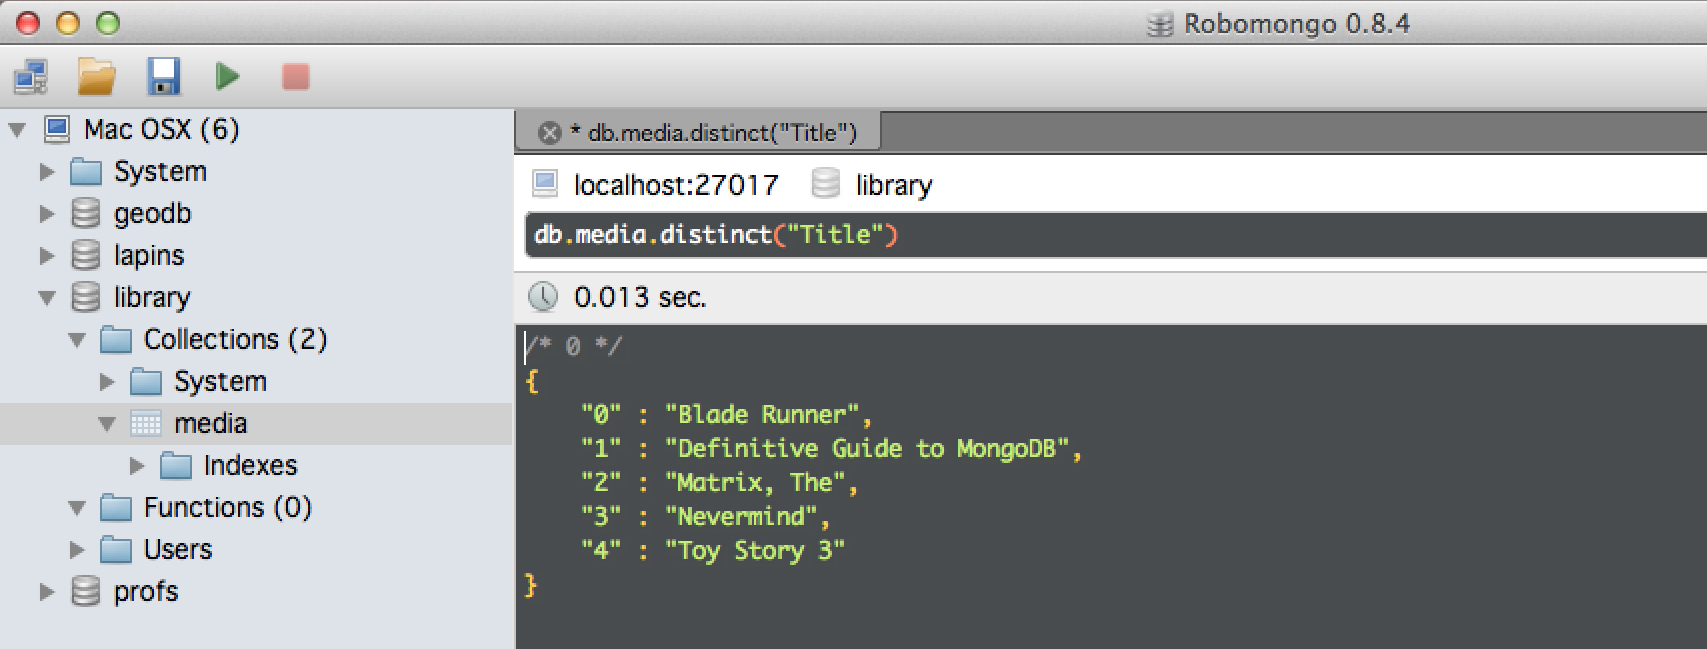
\includegraphics[scale=0.5]{img/distinct.png}
    \caption{Aperçu du tableau Javascripte retourné par la méthode .distinct()}
    \end{figure}
    
    \par Il est également possible de filtrer les documents traités par un .distinct() à l'aide d'un argument optionnel \textbf{query}. La requête suivente contruit alors un tableau de titre distinct uniquement à partir des livres de prix supérieur à 5.\newline
    
    \begin{tt} db.media.distinct("Title",\{price:\{\$gt:5\}\})\end{tt} \newline
    A l'aide des indications sur la méthode .groupe() on essaie de résoudre l'exercice suivant:
    
    \subsection{Exercice, transformer cette requête SQL en requête mongo}
    
    select a,b,sum(c) csum from coll where active=1 group by a,b \newline \newline
    \begin{tt} db.coll.group(\{ key: \{a: true, b: true\},\newline
    \indent cond: \{ active: 1 \}, \newline
    \indent reduce: function(curr, result)\{ \newline
    \indent \indent result.csum += curr.c; \newline
    \indent\}, \newline
    initial: \{csum: 0\} \newline
    \}); \newline \end{tt}
    
{\let\thefootnote\relax\footnotetext{\textsuperscript{3}\textit{\href{http://docs.mongodb.org/manual/reference/method/db.collection.distinct/}{Examples of the db.collection.distinct() method:}}}}
